\documentclass{beamer}
\usepackage{amsfonts,amsmath,oldgerm}
\usepackage{booktabs}
\usepackage{graphicx}
\usepackage{tikz}
\usetikzlibrary{positioning,shapes.geometric}
\usetheme{sintef}

\usefonttheme[onlymath]{serif}

\titlebackground*{assets/background}

\newcommand{\hrefcol}[2]{\textcolor{cyan}{\href{#1}{#2}}}

\title{Audio-Visual Speech Recognition}
\subtitle{Multimodal Interaction Project}
\course{Master's Degree in Computer Science}
\author{Diego Mattias Barreto}
\IDnumber{1901707}
\date{Academic Year 2024/2025}

\begin{document}
\maketitle

\section{Motivation}

\begin{frame}{Why Audio-Visual Speech Recognition?}
  \begin{itemize}
    \item Automatic Speech Recognition (ASR) degrades under real-world noise
    \item The \textbf{cocktail party effect}: overlapping voices mask speech formants
    \item \textbf{Key insight (McGurk effect):} the visual modality --- lip movements --- is \emph{noise-invariant}
    \item AVSR combines audio and video to build a robust, complementary system
  \end{itemize}
  \vspace{0.5em}
  \begin{block}{Goal}
    Classify 10 spoken Italian commands under 6 degradation conditions using an Audio-Visual fusion architecture.
  \end{block}
\end{frame}

\begin{frame}{Project Contributions}
  \begin{enumerate}
    \item \textbf{Multimodal Early Fusion architecture:}\\
          Audio-LSTM + Video-BiLSTM branches fused at feature level
          \vspace{0.4em}
    \item \textbf{Systematic elimination of experimental biases:}\\
          Padding Leakage (Continuous Noise Canvas) and Data Leakage (Stratified Group K-Fold)
          \vspace{0.4em}
    \item \textbf{6-condition Ablation Matrix:}\\
          Empirical validation of modality orthogonality, multimodal synergy, and negative transfer
  \end{enumerate}
\end{frame}

\section{Data \& Features}

\begin{frame}{Dataset}
  \begin{columns}
    \begin{column}{0.55\textwidth}
      \begin{itemize}
        \item \textbf{10 Italian spoken commands:}\\
              \textit{avvia, stop, sopra, sotto,}\\
              \textit{sinistra, destra, apri, chiudi, si, no}
        \item Synchronized \textbf{WAV} (audio) + \textbf{MP4} (video) recordings
        \item Single speaker, controlled environment
        \item Augmentation pipeline:
              \begin{itemize}
                \item Babble Noise at +5\,dB and $-15$\,dB SNR
                \item Spatial Jitter (high-frequency perturbation)
                \item Static Tilt (off-axis framing)
              \end{itemize}
      \end{itemize}
    \end{column}
    \begin{column}{0.45\textwidth}
      \begin{block}{Augmentation Conditions}
        \begin{tabular}{ll}
          \toprule
          \textbf{Modality} & \textbf{Type}    \\
          \midrule
          Audio Light       & +5\,dB Babble    \\
          Audio Heavy       & $-15$\,dB Babble \\
          Video Light       & Jitter           \\
          Video Heavy       & Tilt             \\
          A+V Light         & Both             \\
          \bottomrule
        \end{tabular}
      \end{block}
    \end{column}
  \end{columns}
\end{frame}

\begin{frame}[shrink=5]{Audio Feature Extraction}
  \begin{columns}
    \begin{column}{0.48\textwidth}
      \begin{itemize}
        \item Raw audio resampled to \textbf{16\,kHz}
        \item \textbf{13 MFCCs} computed per frame
        \item Fixed sequence length: \textbf{30 frames}
        \item Input tensor shape: $(30, 13)$
      \end{itemize}
    \end{column}
    \begin{column}{0.48\textwidth}
      \begin{itemize}
        \item \textbf{Why MFCCs?}
              \begin{itemize}
                \item DCT decorrelates spectral envelope
                \item Speaker-independent representation
                \item Isolates phonetic formants from raw energy
              \end{itemize}
      \end{itemize}
    \end{column}
  \end{columns}
  \vspace{0.4em}
  \begin{center}
    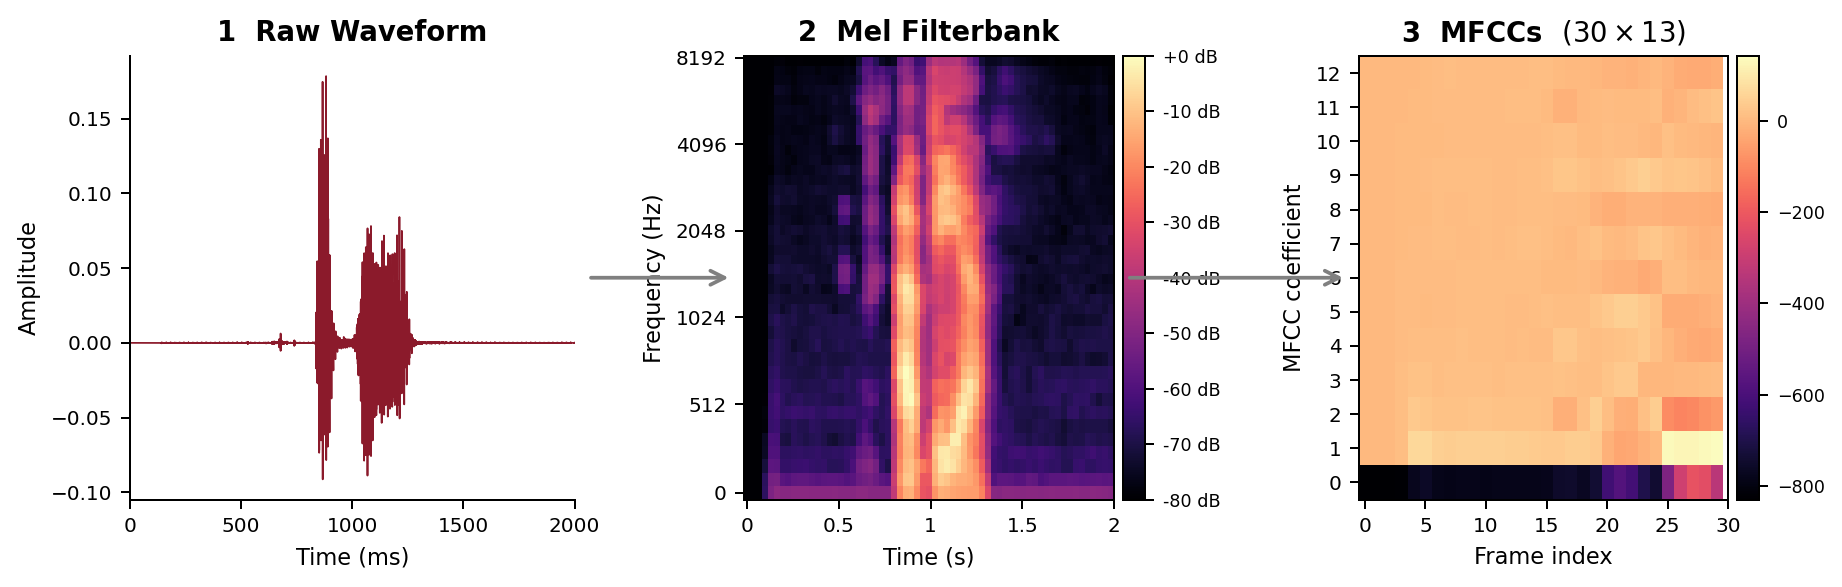
\includegraphics[width=\textwidth,height=0.52\textheight,keepaspectratio]{../report/assets/mfcc_pipeline}
  \end{center}
\end{frame}

\begin{frame}[shrink=5]{Video Feature Extraction}
  \begin{columns}
    \begin{column}{0.48\textwidth}
      \begin{itemize}
        \item \textbf{MediaPipe Face Mesh} detects 3D facial landmarks
        \item 3 static geometric measures per frame:\\
              inner aperture, outer aperture, lip width
        \item \textbf{Problem:} static geometry $\Rightarrow$ gradient stagnation
      \end{itemize}
    \end{column}
    \begin{column}{0.48\textwidth}
      \begin{itemize}
        \item \textbf{Solution:} kinematic derivatives
              \begin{itemize}
                \item $\Delta$ (velocity) and $\Delta\Delta$ (acceleration)
                \item $3 \rightarrow 9$ features per frame
              \end{itemize}
        \item Input tensor shape: $(30, 9)$
      \end{itemize}
    \end{column}
  \end{columns}
  \vspace{0.4em}
  \begin{center}
    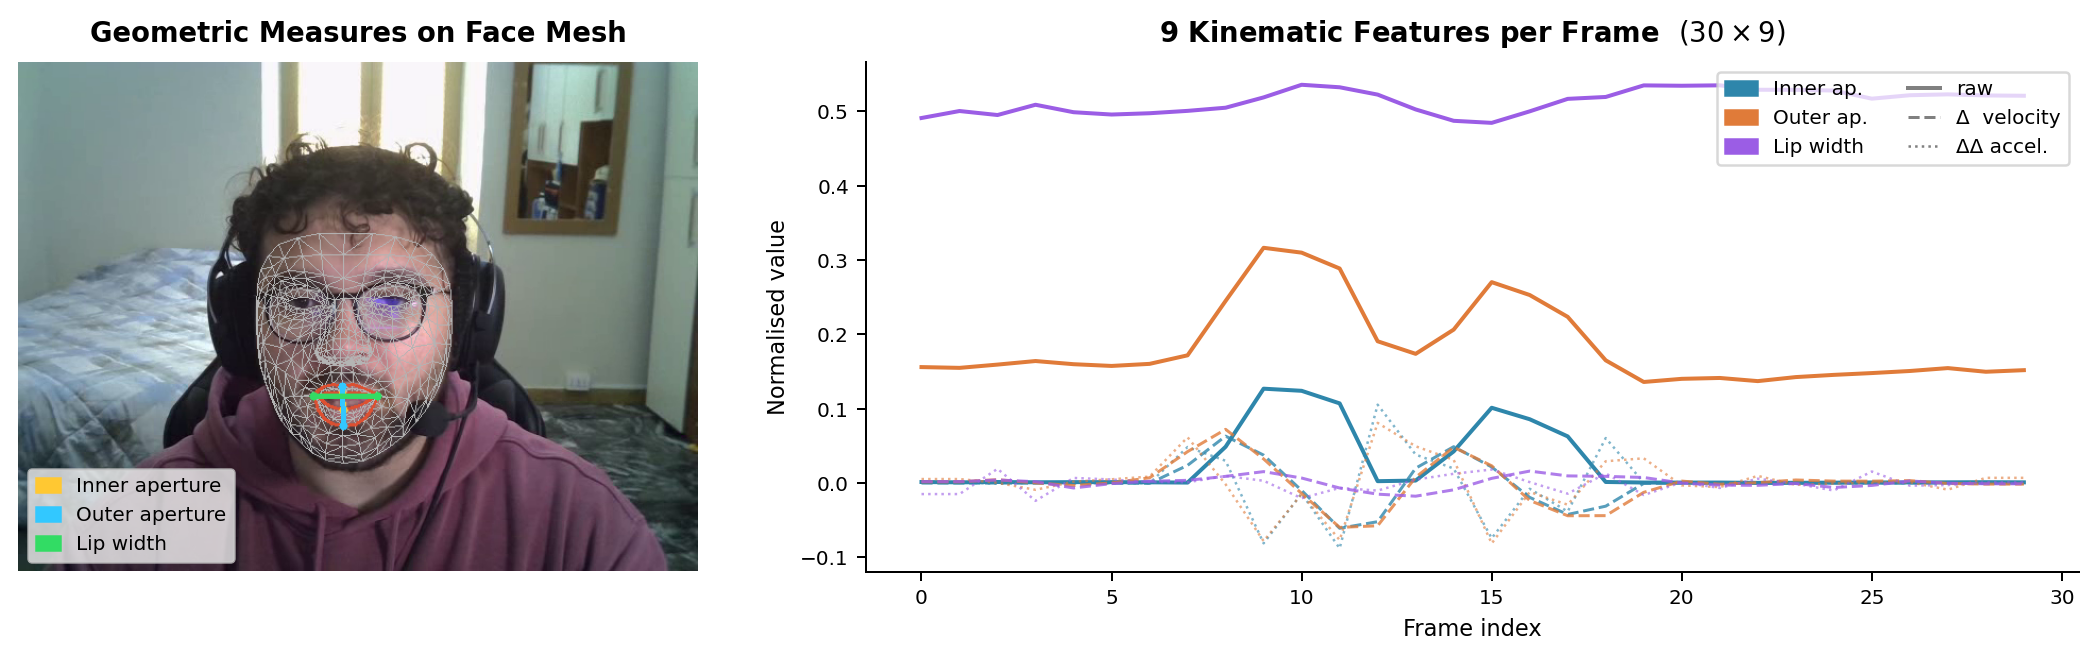
\includegraphics[width=\textwidth,height=0.52\textheight,keepaspectratio]{../report/assets/video_pipeline}
  \end{center}
\end{frame}

\section{Methodology}

\begin{frame}[shrink=5]{Bias \#1: Data Leakage}
  \begin{columns}
    \begin{column}{0.48\textwidth}
      \begin{block}{Problem}
        Random split $\Rightarrow$ augmented variants of the same recording appear in \emph{both} train and test sets.
        Result: \textbf{100\% accuracy} even at $-15$\,dB --- artificially inflated by speaker memorization.
      \end{block}
    \end{column}
    \begin{column}{0.48\textwidth}
      \begin{block}{Solution: Stratified Group K-Fold}
        \begin{enumerate}
          \item \texttt{GroupKFold} ($n{=}7$): carve fixed \textbf{test} set
          \item \texttt{GroupKFold} ($n{=}5$): \textbf{train / val} split
          \item Group $=$ base filename; stratification enforces class balance
        \end{enumerate}
      \end{block}
    \end{column}
  \end{columns}
  \vspace{0.3em}
  \begin{center}
    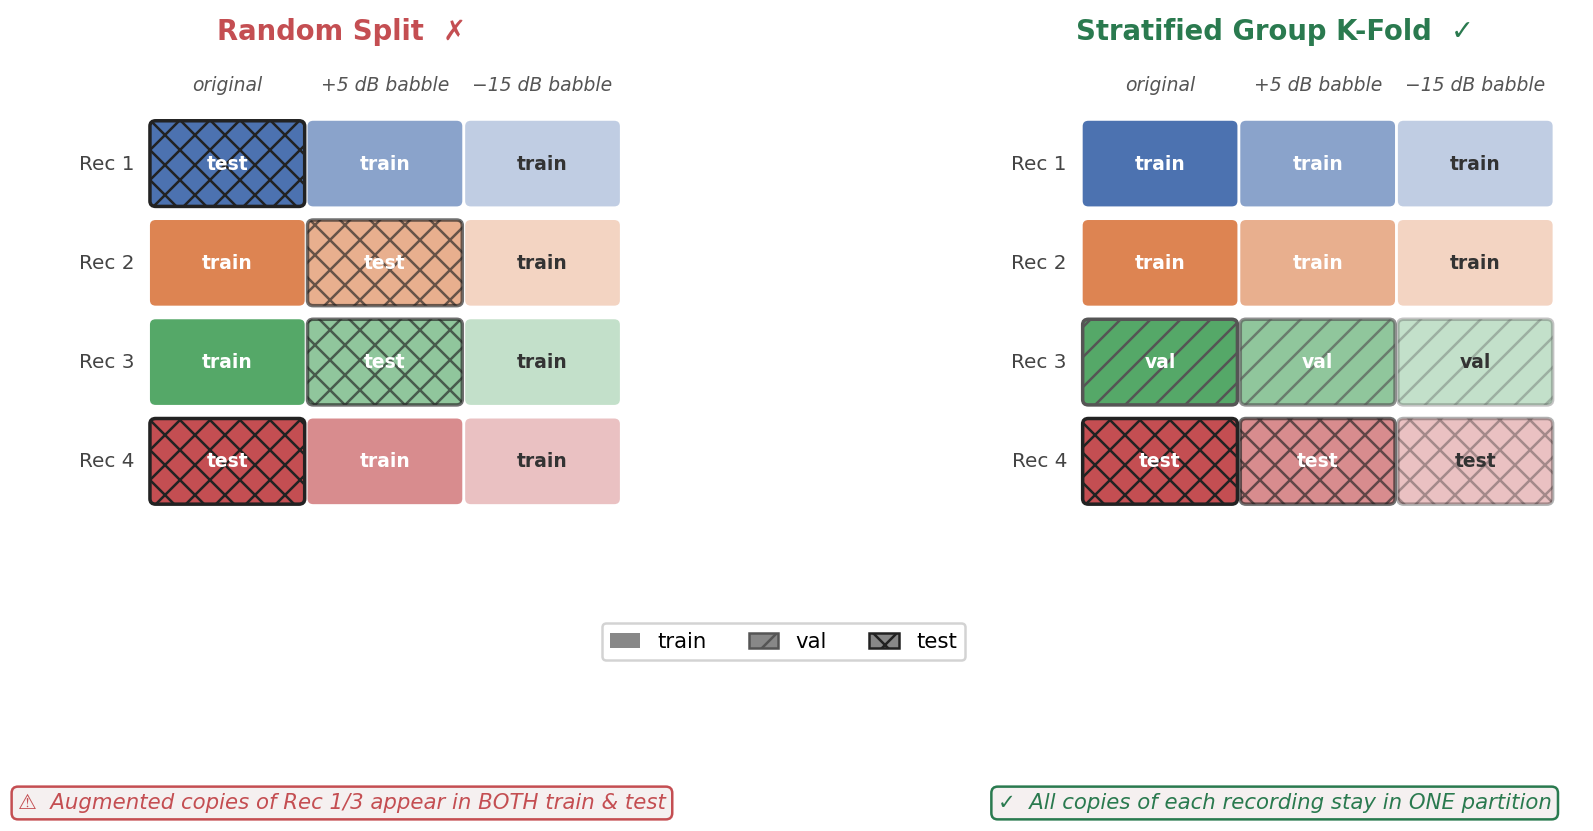
\includegraphics[width=\textwidth,height=0.48\textheight,keepaspectratio]{../report/assets/data_leakage}
  \end{center}
\end{frame}

\begin{frame}[shrink=5]{Bias \#2: Padding Leakage}
  \begin{columns}
    \begin{column}{0.48\textwidth}
      \begin{block}{Problem}
        Zero-padding to 30 frames $\Rightarrow$ LSTM \emph{counts} zero-frames to infer spoken word duration.
        The network bypasses phonetic learning --- it just counts silence.
      \end{block}
    \end{column}
    \begin{column}{0.48\textwidth}
      \begin{block}{Solution: Continuous Noise Canvas}
        \begin{enumerate}
          \item Noise canvas of full target length (30 frames)
          \item Speech waveform at a \textbf{randomized offset}
          \item Every frame contains non-zero acoustic data
        \end{enumerate}
      \end{block}
    \end{column}
  \end{columns}
  \vspace{0.3em}
  \begin{center}
    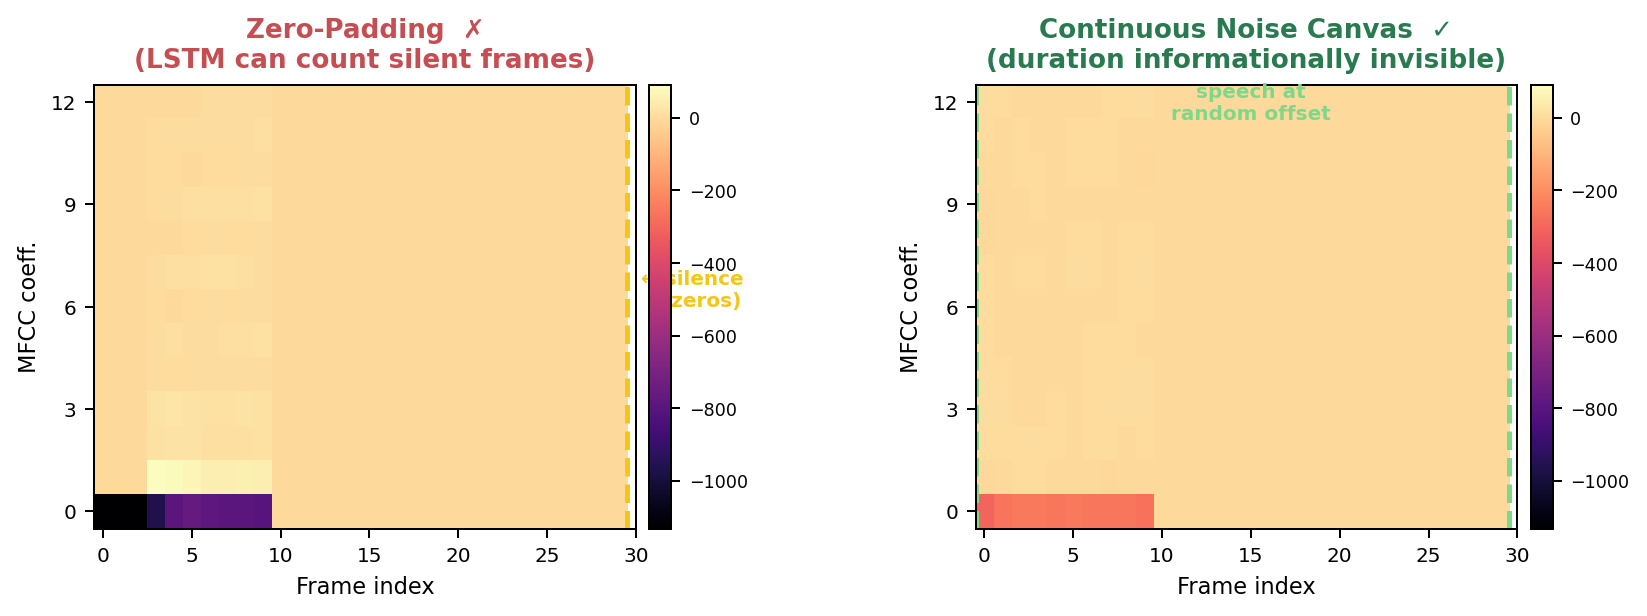
\includegraphics[width=\textwidth,height=0.48\textheight,keepaspectratio]{../report/assets/padding_leakage}
  \end{center}
\end{frame}

\section{Architectures}

\begin{frame}{Audio-Only LSTM}
  \begin{columns}
    \begin{column}{0.42\textwidth}
      \begin{itemize}
        \item Input: $(30, 13)$ MFCC sequence
        \item \textbf{Unidirectional LSTM:} speech formants unfold causally
        \item BatchNorm normalizes MFCCs online during training
      \end{itemize}
    \end{column}
    \begin{column}{0.58\textwidth}
      \centering
      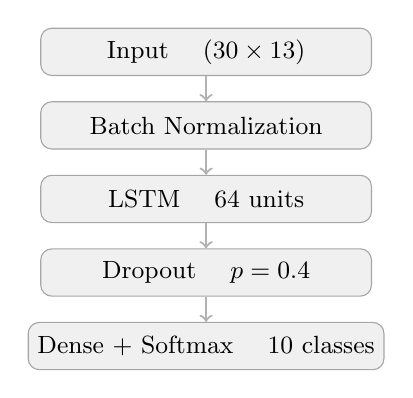
\begin{tikzpicture}[
          box/.style={rectangle, draw=gray!70, rounded corners=4pt,
              fill=gray!12, minimum width=4.2cm, minimum height=0.6cm,
              font=\small, align=center},
          arr/.style={->, thick, gray!60}
        ]
        \node[box] (inp)  {Input \quad $(30 \times 13)$};
        \node[box, below=0.32cm of inp]  (bn)   {Batch Normalization};
        \node[box, below=0.32cm of bn]   (lstm) {LSTM \quad 64 units};
        \node[box, below=0.32cm of lstm] (drop) {Dropout \quad $p = 0.4$};
        \node[box, below=0.32cm of drop] (out)  {Dense + Softmax \quad 10 classes};
        \draw[arr] (inp)  -- (bn);
        \draw[arr] (bn)   -- (lstm);
        \draw[arr] (lstm) -- (drop);
        \draw[arr] (drop) -- (out);
      \end{tikzpicture}
    \end{column}
  \end{columns}
\end{frame}

\begin{frame}{Video-Only BiLSTM}
  \begin{columns}
    \begin{column}{0.42\textwidth}
      \begin{itemize}
        \item Input: $(30, 9)$ kinematic sequence
        \item \textbf{Bidirectional LSTM:} lip movements exhibit coarticulation --- future context is needed
        \item Masking ignores zero-padded frames
      \end{itemize}
    \end{column}
    \begin{column}{0.58\textwidth}
      \centering
      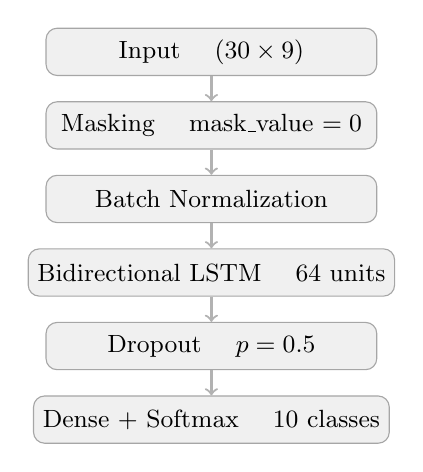
\begin{tikzpicture}[
          box/.style={rectangle, draw=gray!70, rounded corners=4pt,
              fill=gray!12, minimum width=4.2cm, minimum height=0.6cm,
              font=\small, align=center},
          arr/.style={->, thick, gray!60}
        ]
        \node[box] (inp)   {Input \quad $(30 \times 9)$};
        \node[box, below=0.32cm of inp]   (mask) {Masking \quad mask\_value $= 0$};
        \node[box, below=0.32cm of mask]  (bn)   {Batch Normalization};
        \node[box, below=0.32cm of bn]    (lstm) {Bidirectional LSTM \quad 64 units};
        \node[box, below=0.32cm of lstm]  (drop) {Dropout \quad $p = 0.5$};
        \node[box, below=0.32cm of drop]  (out)  {Dense + Softmax \quad 10 classes};
        \draw[arr] (inp)   -- (mask);
        \draw[arr] (mask)  -- (bn);
        \draw[arr] (bn)    -- (lstm);
        \draw[arr] (lstm)  -- (drop);
        \draw[arr] (drop)  -- (out);
      \end{tikzpicture}
    \end{column}
  \end{columns}
\end{frame}

\begin{frame}[shrink=5]{Early Fusion Multimodal Model}
  \small Two parallel branches fused at feature level. The shared Dense layer learns \textbf{cross-modal correlations} (e.g.\ acoustic silence $\leftrightarrow$ lip closure).
  \vspace{0.3em}
  \begin{center}
    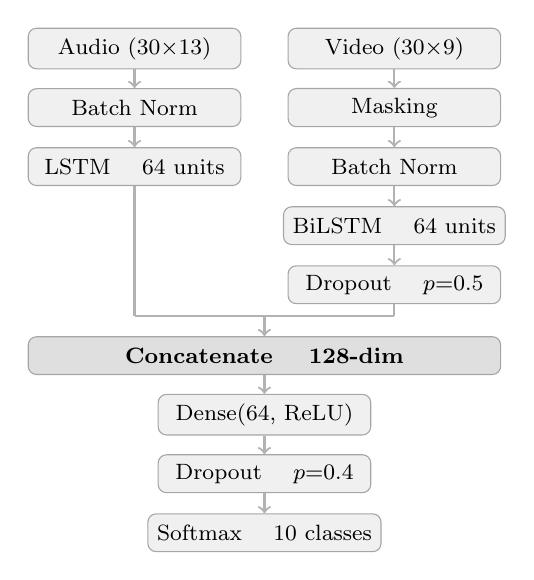
\begin{tikzpicture}[
        box/.style={rectangle, draw=gray!70, rounded corners=3pt,
            fill=gray!12, minimum width=2.7cm, minimum height=0.48cm,
            font=\footnotesize, align=center},
        merge/.style={rectangle, draw=gray!70, rounded corners=3pt,
            fill=gray!25, minimum width=6.0cm, minimum height=0.48cm,
            font=\footnotesize\bfseries, align=center},
        arr/.style={->, thick, gray!60}
      ]
      % Audio branch — absolute coords, x=0
      \node[box] at (0,    0)    (ainp)  {Audio $(30{\times}13)$};
      \node[box] at (0,   -0.75) (abn)   {Batch Norm};
      \node[box] at (0,   -1.50) (alst)  {LSTM \quad 64 units};

      % Video branch — absolute coords, x=3.3
      \node[box] at (3.3,  0)    (vinp)  {Video $(30{\times}9)$};
      \node[box] at (3.3, -0.75) (vmask) {Masking};
      \node[box] at (3.3, -1.50) (vbn)   {Batch Norm};
      \node[box] at (3.3, -2.25) (vlst)  {BiLSTM \quad 64 units};
      \node[box] at (3.3, -3.00) (vdrop) {Dropout \quad $p{=}0.5$};

      % Concatenate — centered, below T-junction at y=-3.40
      \node[merge] at (1.65, -3.90) (cat) {Concatenate \quad 128-dim};

      % Shared head
      \node[box] at (1.65, -4.65) (dense) {Dense(64, ReLU)};
      \node[box] at (1.65, -5.40) (drop2) {Dropout \quad $p{=}0.4$};
      \node[box] at (1.65, -6.15) (out)   {Softmax \quad 10 classes};

      % Audio arrows
      \draw[arr] (ainp) -- (abn);
      \draw[arr] (abn)  -- (alst);

      % Video arrows
      \draw[arr] (vinp)  -- (vmask);
      \draw[arr] (vmask) -- (vbn);
      \draw[arr] (vbn)   -- (vlst);
      \draw[arr] (vlst)  -- (vdrop);

      % T-junction: both branches go straight down to y=-3.40, then horizontal bar, then arrow to cat
      \draw[thick,gray!60] (alst.south)  -- (0,   -3.40);
      \draw[thick,gray!60] (vdrop.south) -- (3.3, -3.40);
      \draw[thick,gray!60] (0, -3.40)    -- (3.3, -3.40);
      \draw[arr]           (1.65, -3.40) -- (cat.north);

      % Shared head arrows
      \draw[arr] (cat)   -- (dense);
      \draw[arr] (dense) -- (drop2);
      \draw[arr] (drop2) -- (out);
    \end{tikzpicture}
  \end{center}
\end{frame}

\section{Results}

\begin{frame}[shrink=5]{Ablation Matrix}
  \begin{center}
    \footnotesize
    \begin{tabular}{lcccccc}
      \toprule
      \textbf{Model}        & \textbf{Clean} & \textbf{Aud.\ L} & \textbf{Aud.\ H} & \textbf{Vid.\ L} & \textbf{Vid.\ H} & \textbf{A+V L}   \\
      \midrule
      Audio LSTM            & 100\%          & 100\%            & 44.83\%          & 100\%            & 100\%            & 96.55\%          \\
      Video BiLSTM          & 96.55\%        & 96.55\%          & 96.55\%          & 41.38\%          & 96.55\%          & 34.48\%          \\
      \textbf{Early Fusion} & \textbf{100\%} & \textbf{100\%}   & \textbf{86.21\%} & \textbf{96.55\%} & \textbf{100\%}   & \textbf{96.55\%} \\
      \bottomrule
    \end{tabular}
  \end{center}
  \vspace{0.4em}
  \begin{itemize}
    \item Aud.\ L/H = Babble Noise at +5\,dB / $-15$\,dB SNR
    \item Vid.\ L/H = Spatial Jitter / Static Tilt
    \item A+V L = simultaneous +5\,dB noise + Jitter
    \item \textbf{Overall:} Fusion \textbf{96.55\%} $>$ Audio 90.23\% $>$ Video 77.01\%
  \end{itemize}
\end{frame}

\begin{frame}{Multimodal Synergy \& Dynamic Gating}
  \begin{columns}
    \begin{column}{0.5\textwidth}
      \begin{block}{Audio Recovery (Aud.\ Heavy)}
        \begin{itemize}
          \item Audio LSTM: \alert{44.83\%}
          \item Early Fusion: \textbf{86.21\%}
          \item Recovery: $\mathbf{+41.38}$ pp
        \end{itemize}
        Visual features act as an anchor when audio is catastrophically degraded.
      \end{block}
    \end{column}
    \begin{column}{0.5\textwidth}
      \begin{block}{Video Recovery (Vid.\ Light)}
        \begin{itemize}
          \item Video BiLSTM: \alert{41.38\%}
          \item Early Fusion: \textbf{96.55\%}
          \item Recovery: $\mathbf{+55.17}$ pp
        \end{itemize}
        Network ignores corrupted kinematics and relies entirely on clean audio.
      \end{block}
    \end{column}
  \end{columns}
  \vspace{0.5em}
  \begin{itemize}
    \item \textbf{A+V Light:} fusion achieves 96.55\% --- no negative transfer, but no synergy when \emph{both} channels are degraded simultaneously
  \end{itemize}
\end{frame}

\begin{frame}[shrink=5]{Learning Curves}
  \begin{columns}
    \begin{column}{0.33\textwidth}
      \centering
      \textbf{Audio LSTM}\\[0.3em]
      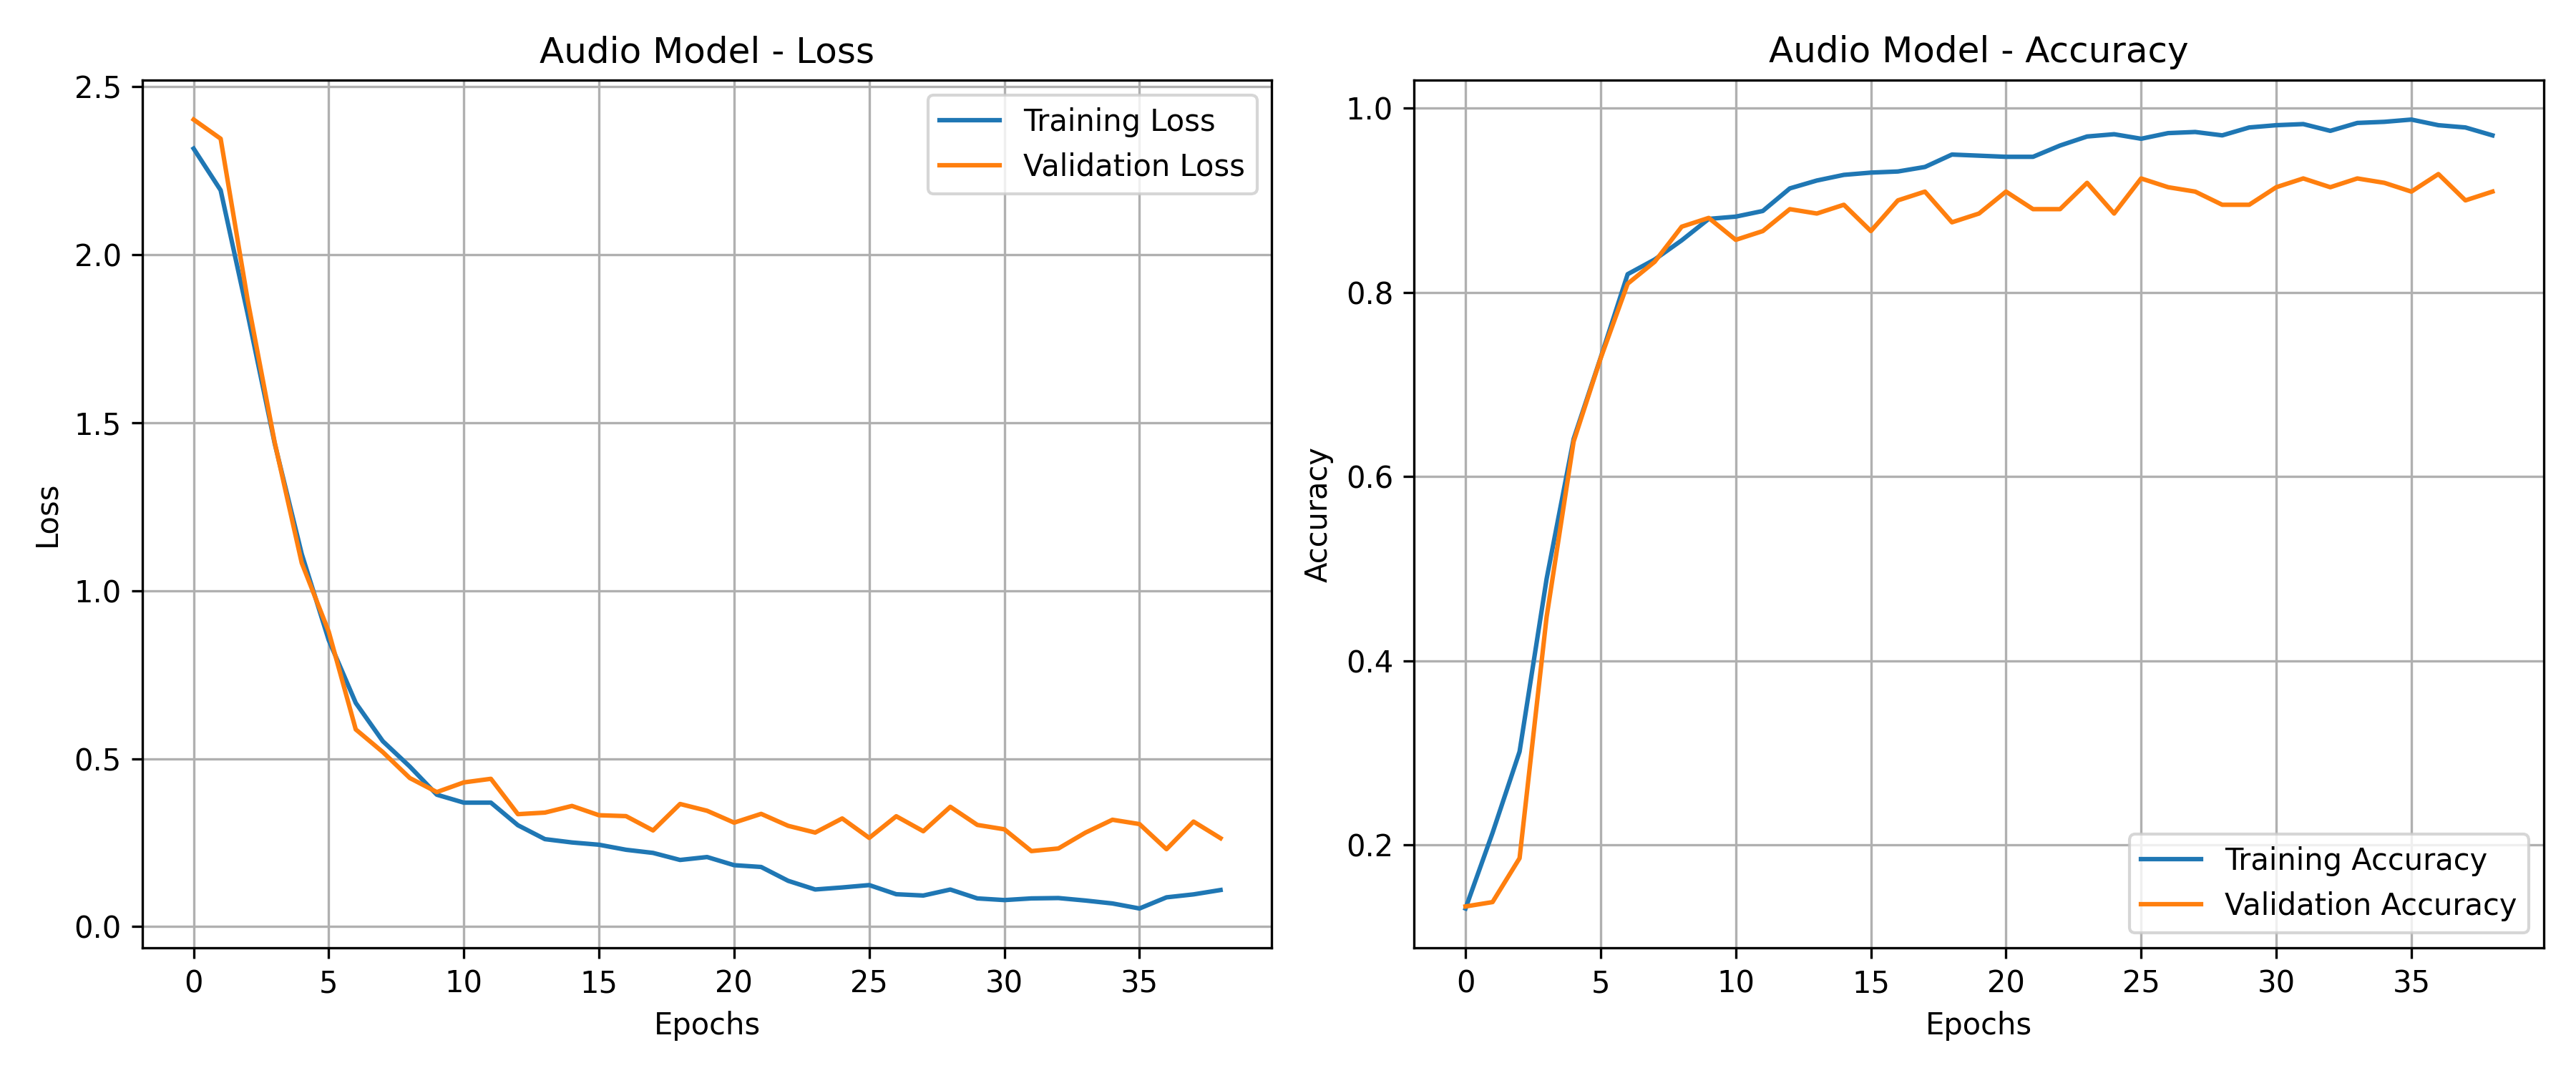
\includegraphics[width=\textwidth,height=0.45\textheight,keepaspectratio]{../report/assets/audio_learning_curves}
    \end{column}
    \begin{column}{0.33\textwidth}
      \centering
      \textbf{Video BiLSTM}\\[0.3em]
      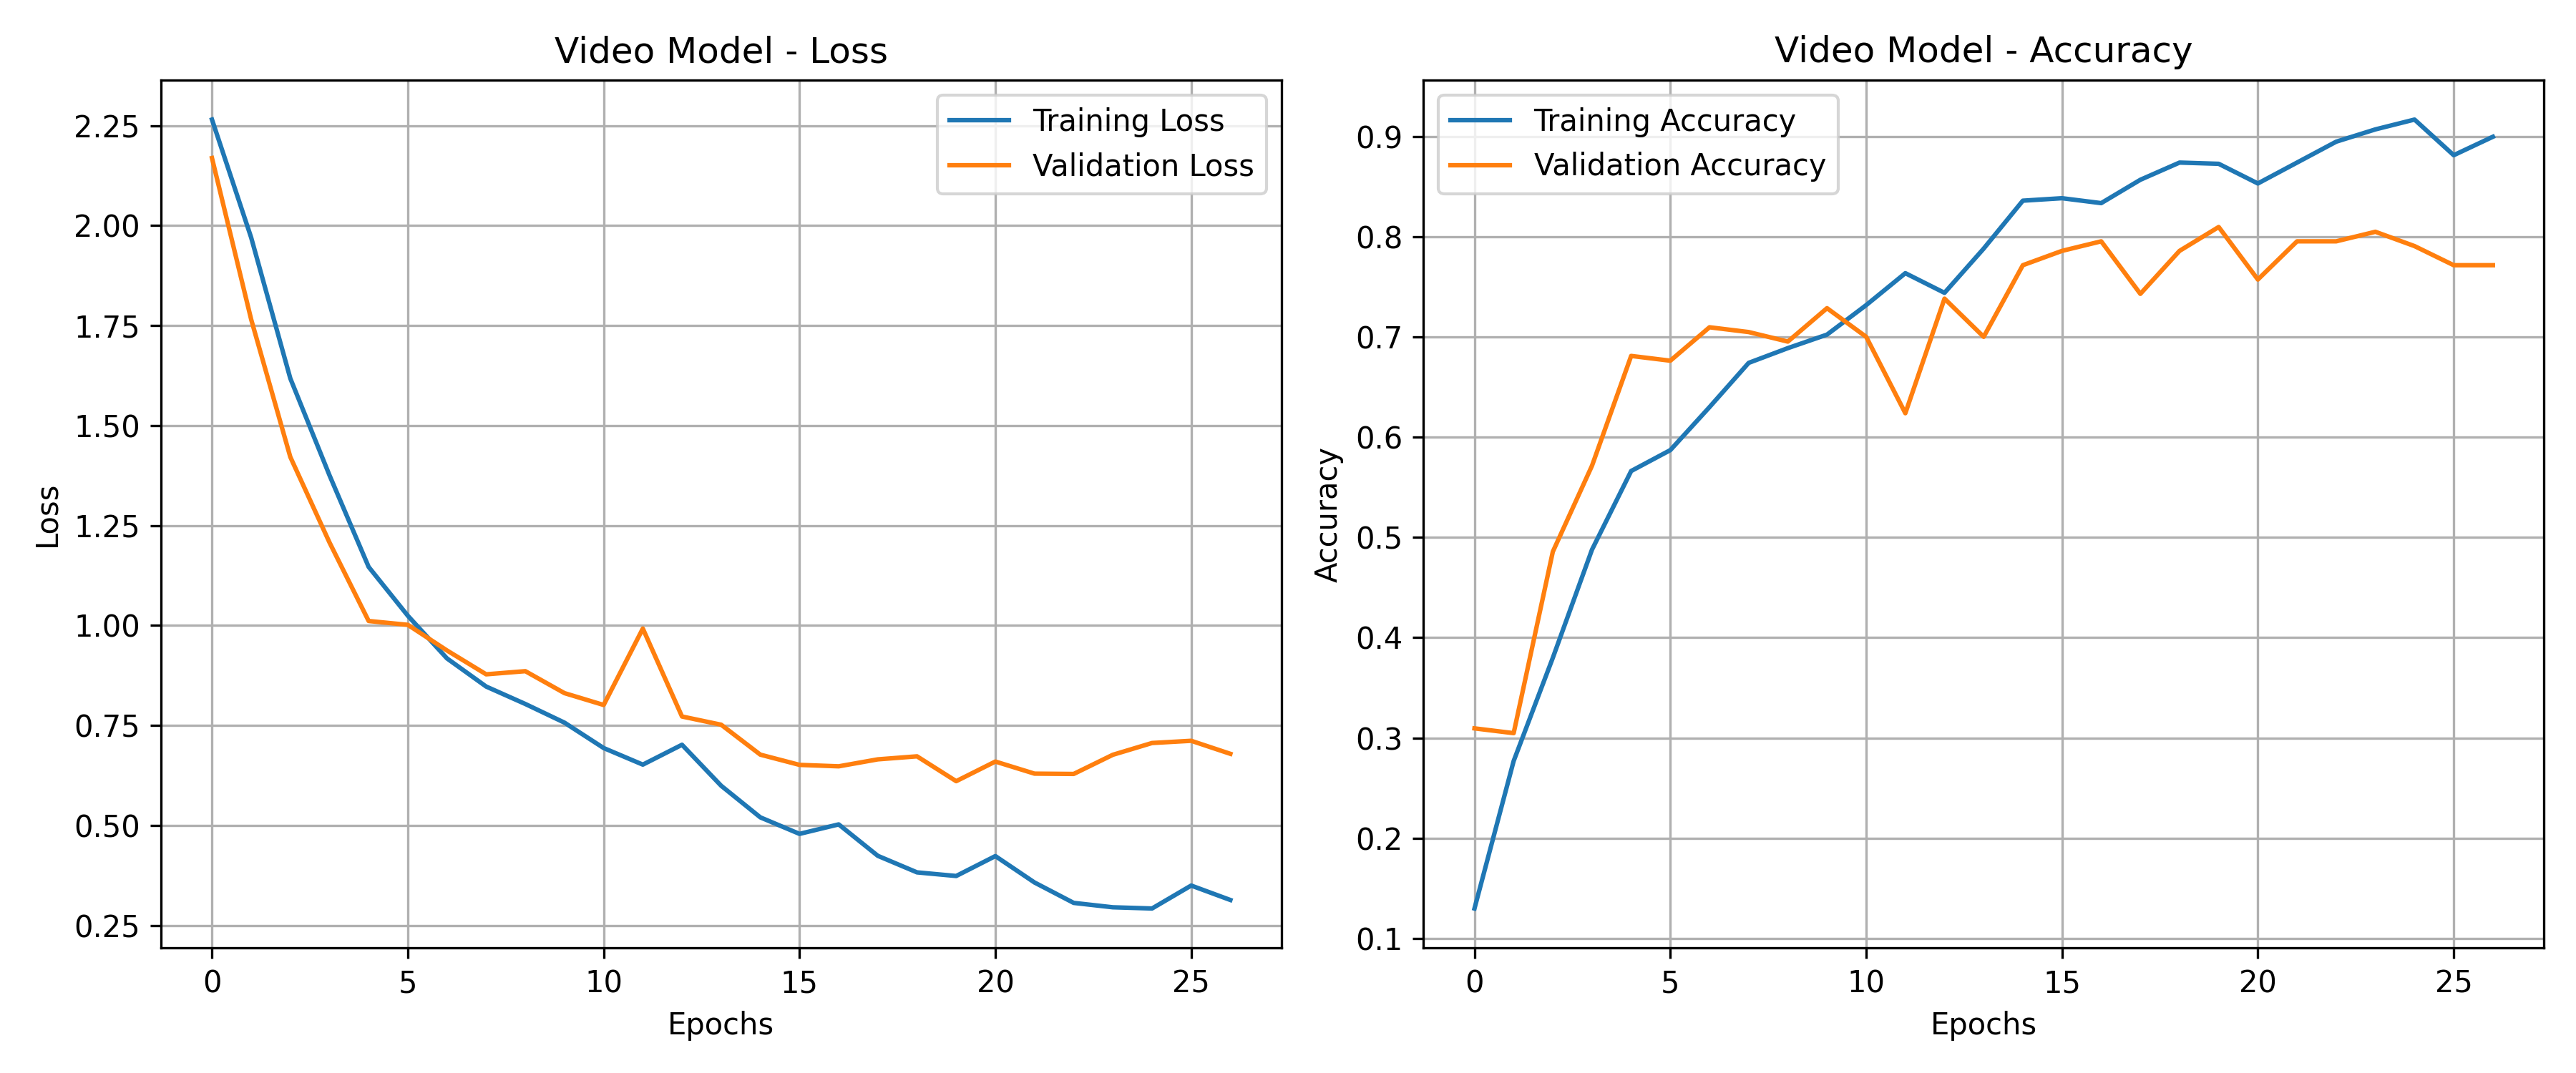
\includegraphics[width=\textwidth,height=0.45\textheight,keepaspectratio]{../report/assets/video_learning_curves}
    \end{column}
    \begin{column}{0.33\textwidth}
      \centering
      \textbf{Early Fusion}\\[0.3em]
      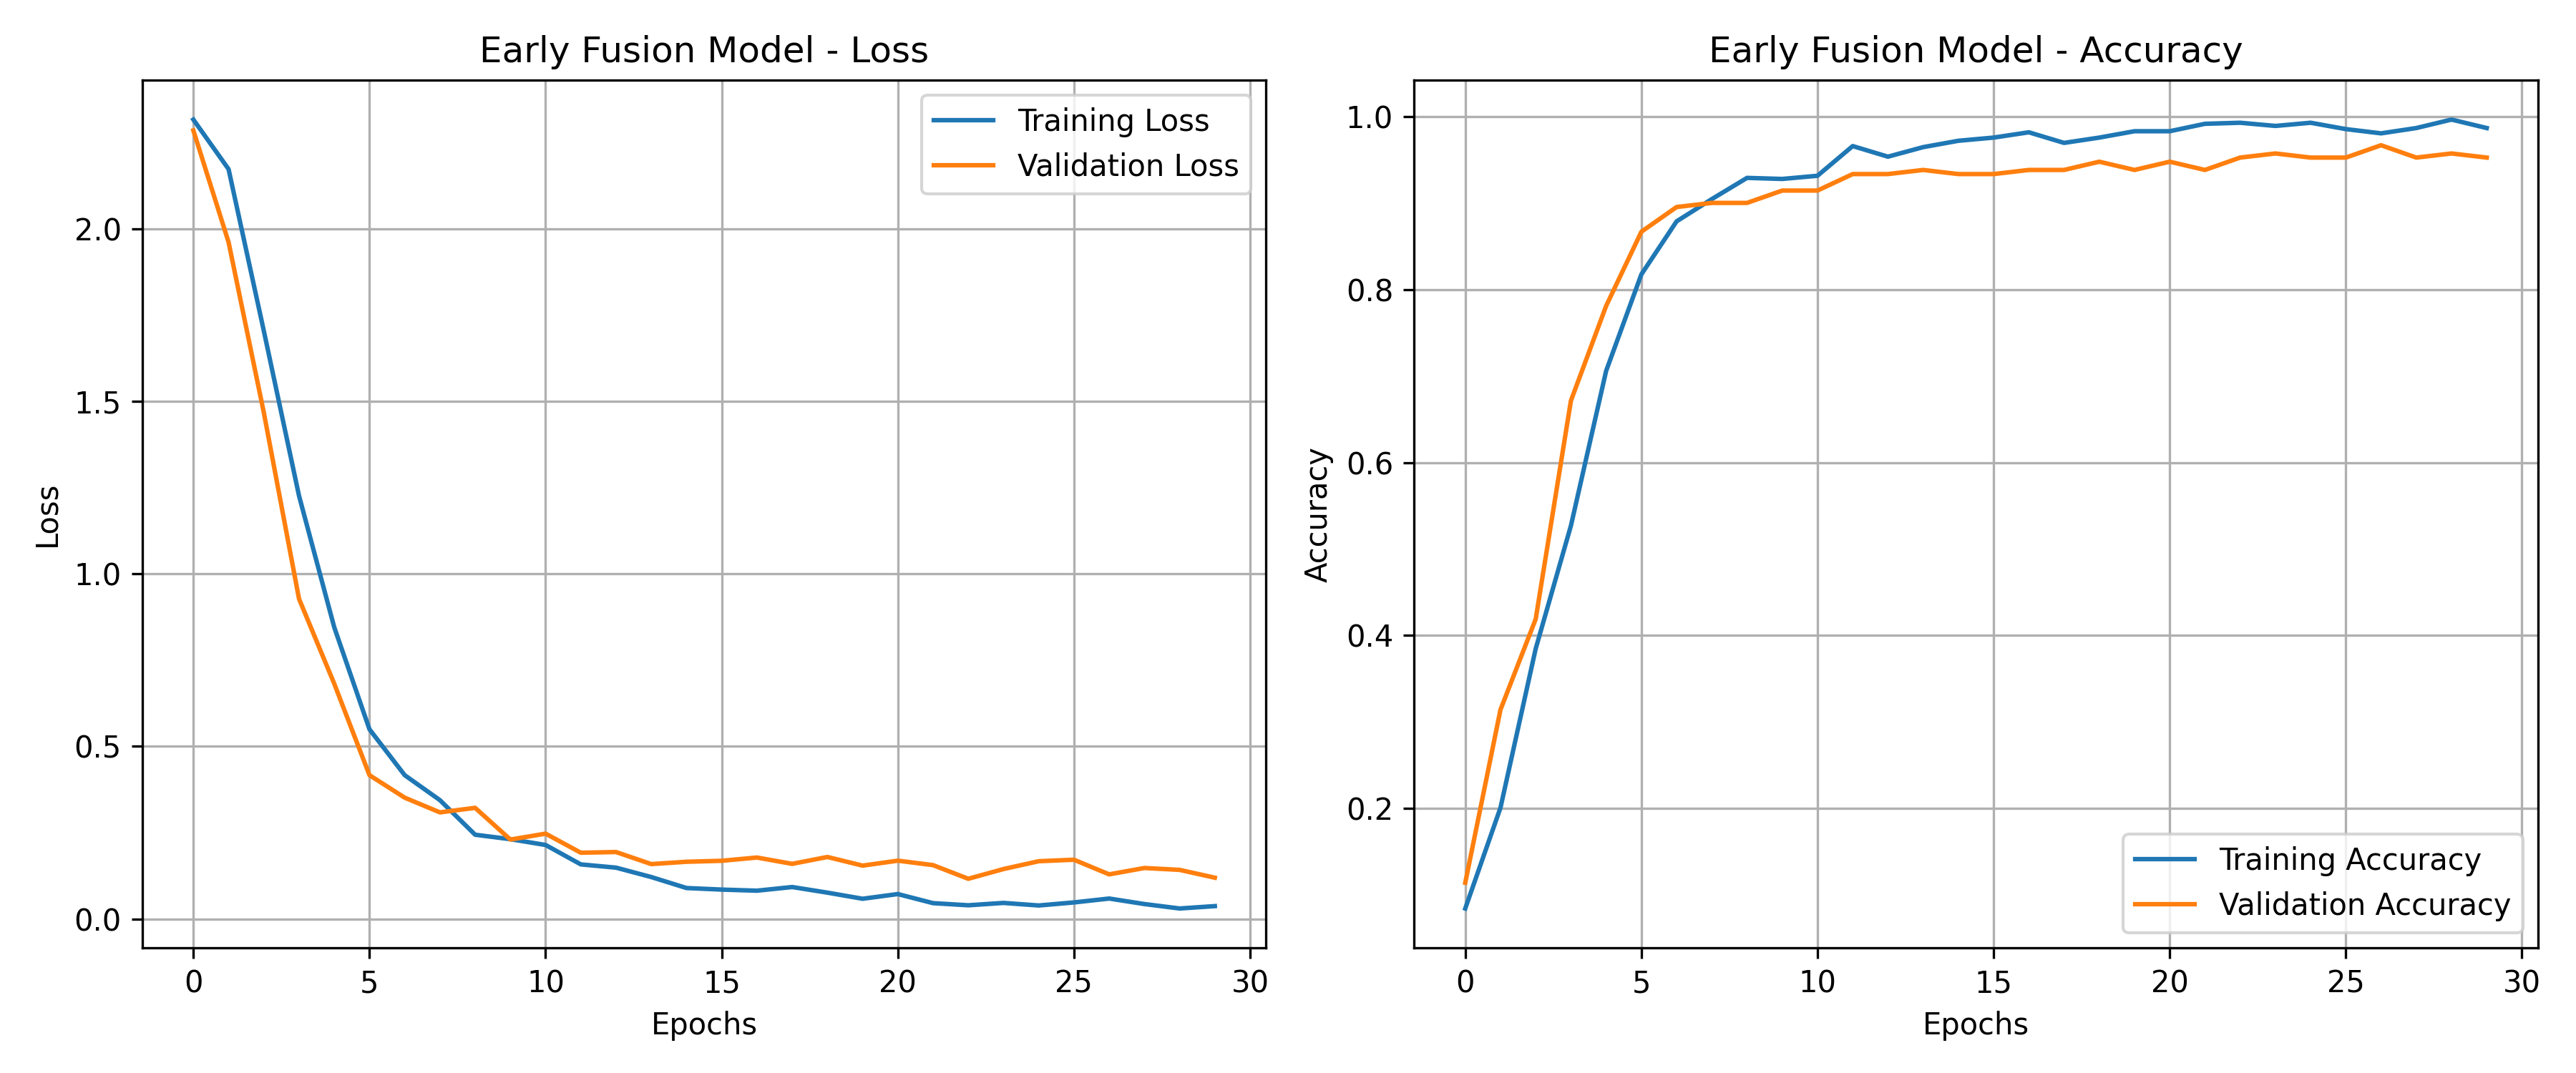
\includegraphics[width=\textwidth,height=0.45\textheight,keepaspectratio]{../report/assets/fusion_learning_curves}
    \end{column}
  \end{columns}
  \vspace{0.4em}
  \begin{itemize}
    \item \textbf{Audio:} stable convergence, val accuracy tracks training closely
    \item \textbf{Video:} slower and noisier convergence --- geometric features carry less signal
    \item \textbf{Fusion:} fastest convergence --- complementary modalities simplify the classification task
  \end{itemize}
\end{frame}

\begin{frame}[shrink=5]{Confusion Matrices}
  \begin{columns}
    \begin{column}{0.33\textwidth}
      \centering
      \textbf{Audio LSTM}\\[0.3em]
      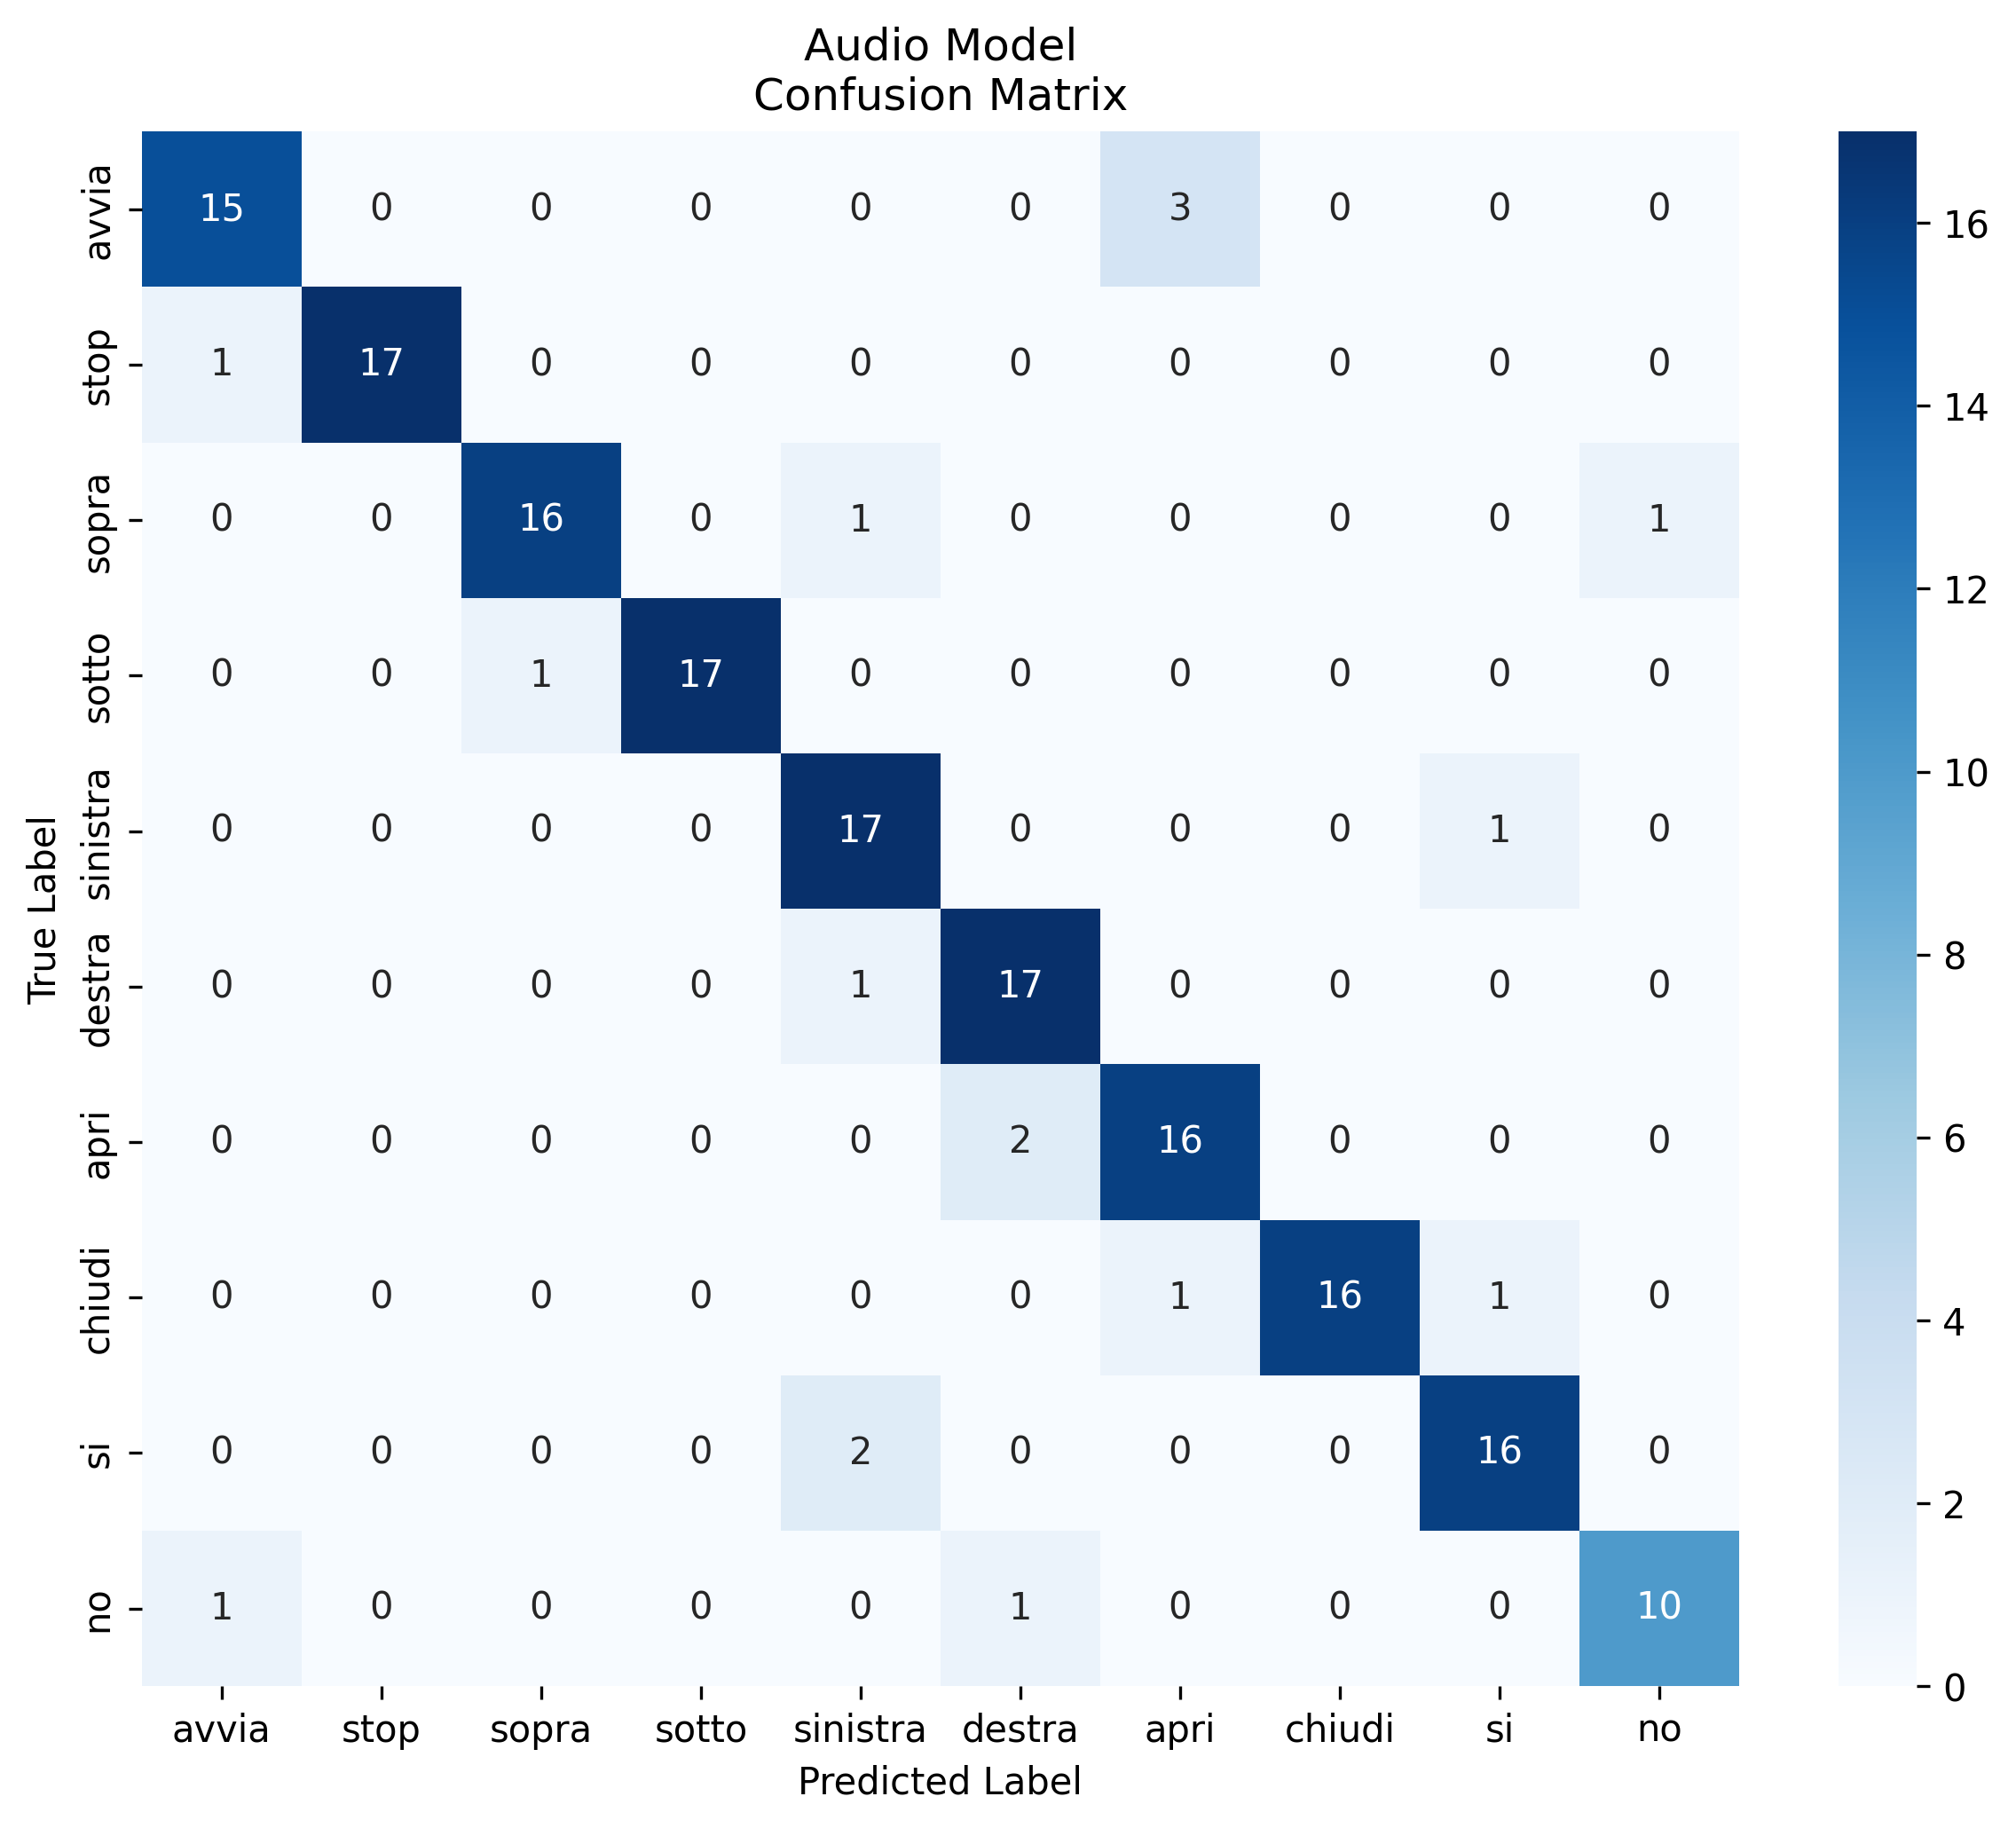
\includegraphics[width=\textwidth,height=0.45\textheight,keepaspectratio]{../report/assets/audio_confusion_matrix}
    \end{column}
    \begin{column}{0.33\textwidth}
      \centering
      \textbf{Video BiLSTM}\\[0.3em]
      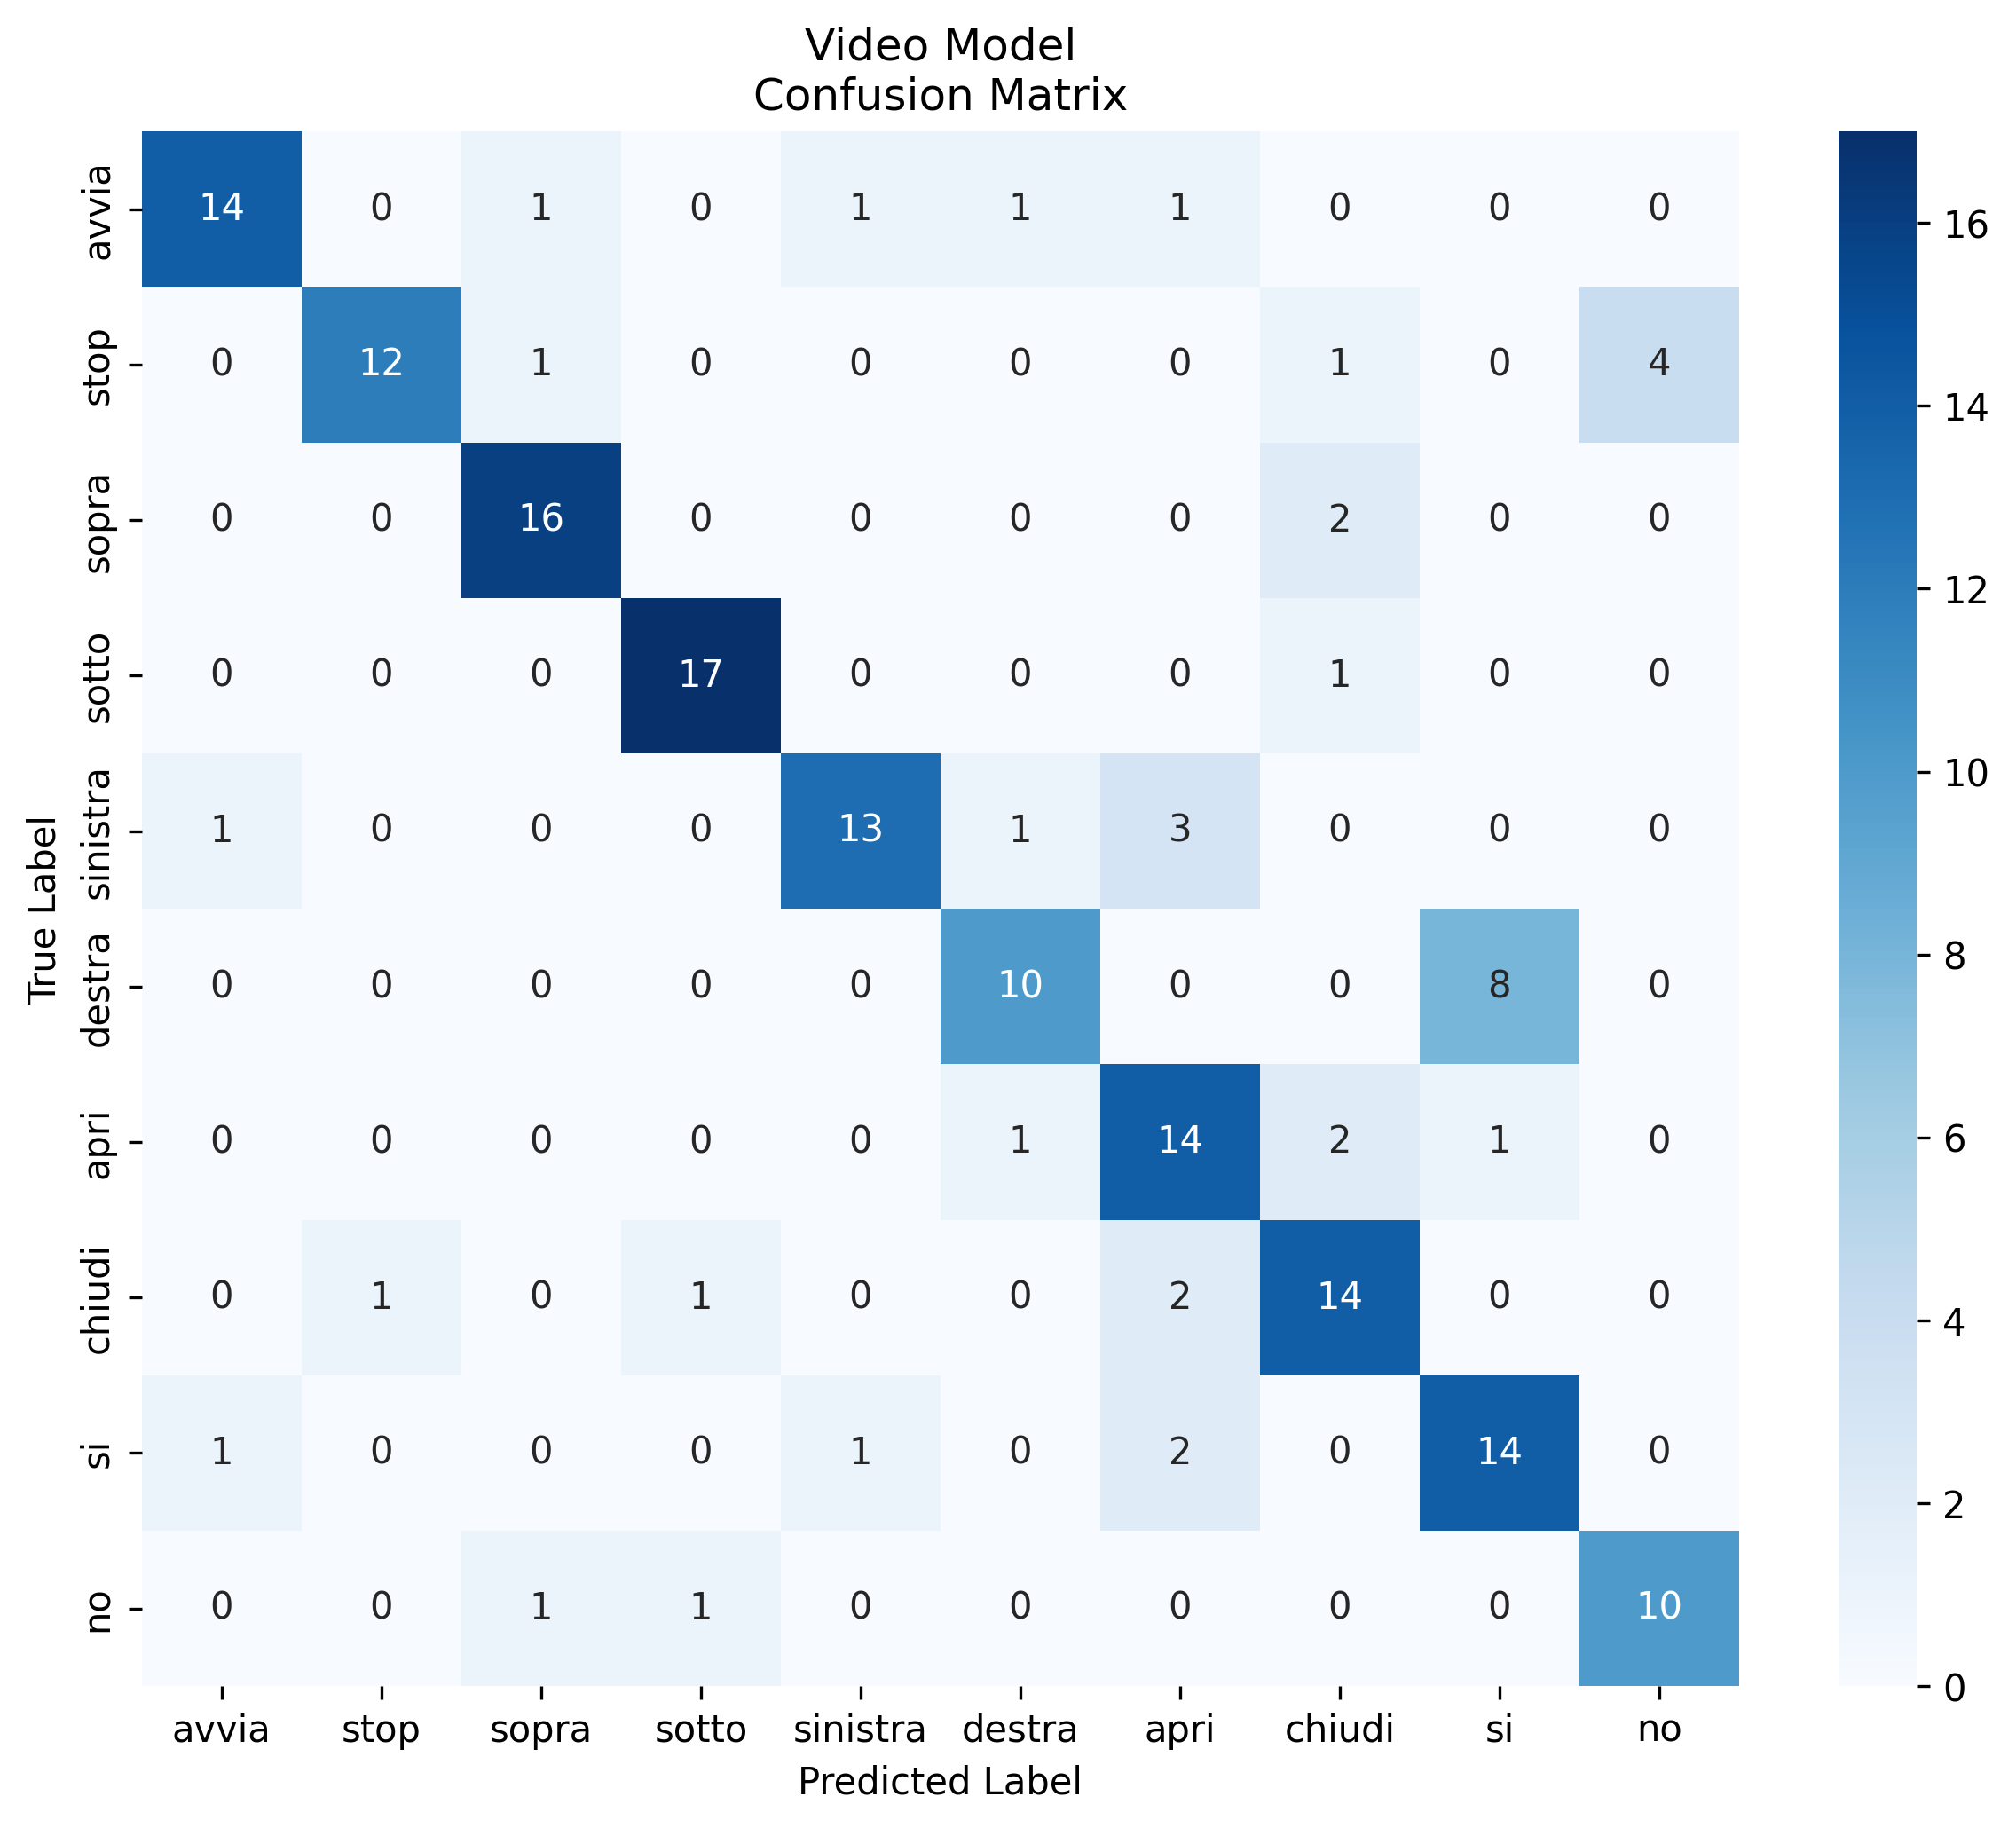
\includegraphics[width=\textwidth,height=0.45\textheight,keepaspectratio]{../report/assets/video_confusion_matrix}
    \end{column}
    \begin{column}{0.33\textwidth}
      \centering
      \textbf{Early Fusion}\\[0.3em]
      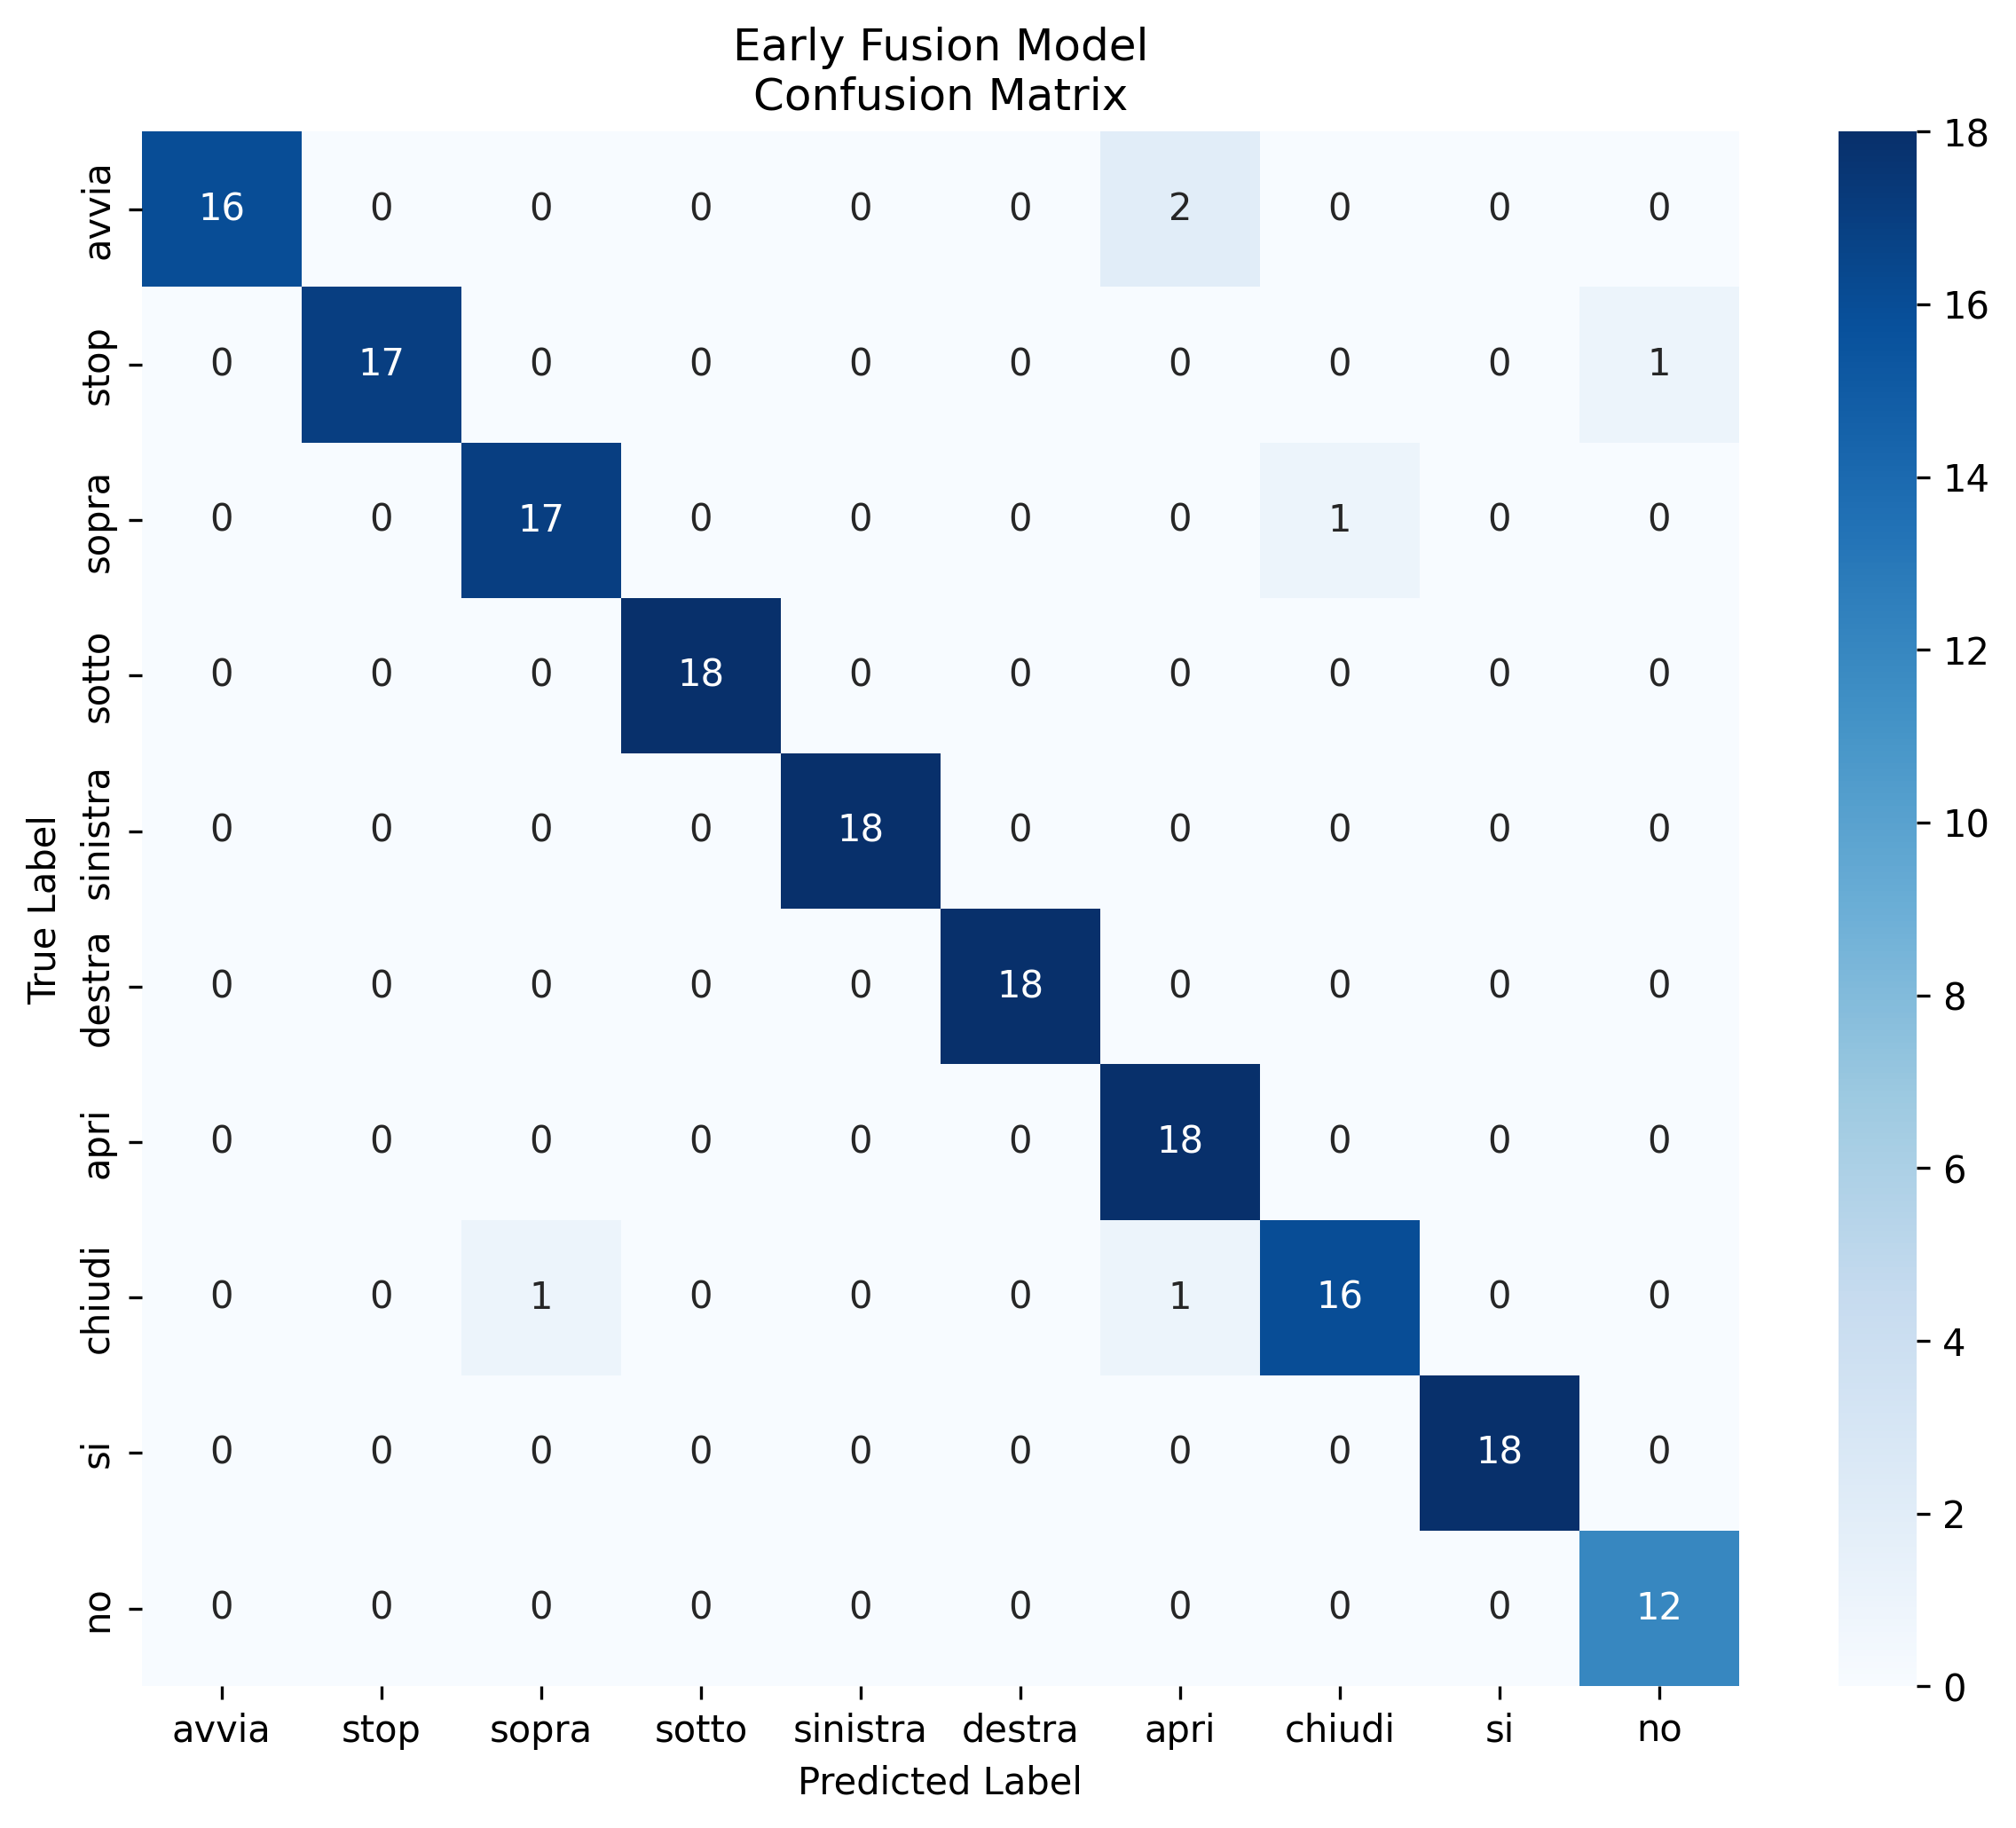
\includegraphics[width=\textwidth,height=0.45\textheight,keepaspectratio]{../report/assets/fusion_confusion_matrix}
    \end{column}
  \end{columns}
  \vspace{0.4em}
  \begin{itemize}
    \item Audio errors cluster in \textbf{Aud.\ Heavy} condition ($-15$\,dB destroys formants)
    \item Video errors cluster in \textbf{Vid.\ Light} (Jitter destroys $\Delta/\Delta\Delta$ derivatives)
    \item Fusion has the \textbf{cleanest diagonal} --- residual errors only in Aud.\ Heavy
  \end{itemize}
\end{frame}

\section{Conclusions}

\begin{frame}[shrink=5]{Conclusions \& Future Work}
  \begin{columns}
    \begin{column}{0.55\textwidth}
      \textbf{Results}
      \begin{itemize}
        \item Early Fusion: \textbf{96.55\%} overall accuracy
        \item Audio-Only: 90.23\% \quad Video-Only: 77.01\%
        \item Visual modality provides \textbf{+41\,pp recovery} under $-15$\,dB babble noise
        \item No negative transfer observed
      \end{itemize}
      \vspace{0.4em}
      \textbf{Limitations}
      \begin{itemize}
        \item Single speaker, controlled environment
        \item Simple concatenation (Early Fusion) cannot dynamically gate per-frame attention
      \end{itemize}
    \end{column}
    \begin{column}{0.45\textwidth}
      \begin{block}{Future Work}
        \begin{itemize}
          \item \textbf{Cross-Modal Attention} and Transformer-based architectures for dynamic per-frame weighting
          \item Expand to multi-speaker, continuous speech vocabulary
          \item Edge deployment via model quantization
        \end{itemize}
      \end{block}
    \end{column}
  \end{columns}
\end{frame}

\backmatter
\end{document}
